\vspace{-10pt}
\section{Evaluation}
\vspace{-10pt}
Our experiments address three questions: (i)~Does \cufuse{} improve latency over host-orchestrated NCCL on diverse compute--communication kernels? (ii)~How does automated co-design compare to an expert-tuned stack (DeepEP, Section~\ref{sec:deepep-comparison})? (iii)~Which pipeline components matter (Section~\ref{sec:ablation})?

The primary quantitative comparisons are \cufuse{} vs.\ host-driven baselines that mirror realistic user code: CPU-launched NCCL collectives and streams as typically written before device-initiated redesign. We implement these host paths with strong conventional overlap---multi-stream scheduling, established collective patterns, and padding only where required---reflecting the most efficient NCCL-centric usage for each workload.

% Expert-library comparisons are workload-specific and appear where we have a runnable counterpart (MoE / DeepEP; Section~\ref{sec:deepep-comparison}).

\noindent\textbf{Benchmarks and workload scope.}
There is, to our knowledge, no public benchmark or dataset of \emph{distributed} multi-GPU programs that jointly exercises computation and communication co-design across heterogeneous topologies. Kernel-generation benchmarks such as KernelBench~\cite{ouyang2025kernelbenchllmswriteefficient} focus on single-GPU tasks rather than multi-GPU programs under varied interconnects. We therefore evaluate on four workloads we construct to cover dominant LLM-side patterns: ring-style attention with repeated peer exchanges (long-context parallelism); MoE dispatch/combine with All-to-All traffic and skewed expert routing; KV handoff for disaggregated prefill--decode serving; and GEMM~+~AllGather as a minimal post-compute collective. Together they span ring, All-to-All, point-to-point handoff, and AllGather semantics.

\noindent\textbf{Environment Setup.} Experiments were conducted across two servers, each featuring dual 16-core Intel Xeons, 256 GiB RAM, and 4x 80 GiB NVIDIA A100 GPUs. Intra-node communication relies on NVLink, and inter-node communication uses RoCE. The system runs Ubuntu 22.04.4 (Linux 5.15), utilizing CUDA 13.1 and NCCL 2.28.9. All LLM agents use Anthropic's Claude Sonnet 4.5.

\noindent\textbf{Search Cost.} For each workload, the slow-path agent evaluates candidates through the three-level cascade over a fixed budget. Across all workloads, the fast-path required 2--3 iterations and the slow-path 10--20 generations, taking 0.8--1.8 hours of wall time and costing \$4.98--\$10.96 in LLM API fees---far less than the hardware cost of the workloads being optimized. A per-workload breakdown is provided in Table~\ref{tab:search-cost} (Appendix~\ref{sec:search-cost-details}).

\noindent\textbf{Workloads.} We evaluate on four workloads that cover dominant LLM communication patterns; Figures~\ref{fig:flash-attn}--\ref{fig:gemm-allgather} summarize end-to-end results. Table~\ref{tab:strategy} previews the co-design strategy \cufuse{} discovered for each workload and the design-space choices that realize it.

\noindent\underline{\emph{Flash Attention with Context Parallelism.}}
This workload implements Ring Attention~\cite{liu2024ringattention}, where each GPU owns one Q shard while KV shards rotate. The bottleneck is inter-round pipeline bubbles. We evaluate on 4 intra-node GPUs (NVLink) with $\text{SEQ} \in \{4096, 8192\}$ and $\text{HD} \in \{32, 64\}$.

\noindent\underline{\emph{DeepSeek-V3 MoE Dispatch and Combine.}}
Each GPU routes tokens to remote experts via AlltoAll dispatch, runs expert GEMMs, and gathers results via a reverse AlltoAll combine. The bottleneck is sequential comm-compute phases and padding overhead under imbalanced routing. We evaluate on 2~GPUs across inter-node RoCE links with 4096~tokens per rank under four skew ratios (2:1 to 5:1).

\noindent\underline{\emph{KV-Cache Transfer.}}
In disaggregated prefill-decode serving, the prefill GPU must compute and send K and V projections before decode can begin. The bottleneck is the compute-to-send idle gap from CPU-launched transfers. We evaluate on two NVLink-connected GPUs with hidden dimension 4096.

\noindent\underline{\emph{GEMM + AllGather.}}
Each rank performs a local GEMM and then participates in an AllGather to distribute the full output. This isolates the simplest post-compute collective with no cross-rank dependencies. We evaluate on 4x GPUs spanning intra-node (NVLink) and inter-node (RoCE) links.

\noindent Full workload details, host baselines and CUCo-discovered pipelines, are provided in Appendix~\ref{sec:workload_details}.

\begin{table*}[t]
\centering
\scriptsize
\setlength{\tabcolsep}{4pt}
\caption{What \cufuse{}'s agent discovered: per-workload dominant bottleneck, the co-design strategy the evolutionary search converged on, and the key design-space choices ($\mathcal{C}$) that realize it.}
% \vspace{-4pt}
\label{tab:strategy}
\begin{tabular}{@{}p{0.10\textwidth}p{0.24\textwidth}p{0.37\textwidth}p{0.20\textwidth}@{}}
\toprule
\textbf{Workload} & \textbf{Dominant bottleneck} & \textbf{Discovered strategy} & \textbf{Key design choices} \\
\midrule
Flash Attention & Pipeline bubbles between ring exchange rounds & Persistent cooperative kernel with per-tile pipelining; comm block polls tile readiness via atomics & $\mathcal{P}$: tile-fused; $\mathcal{M}$: counter; $\mathcal{I}$: CTA (1 comm + 80 compute) \\
MoE Dispatch/ Combine & Sequential comm--compute phases; padding overhead on imbalanced ranks & Self/remote compute split with two-stream dispatch overlap; variable-size per-peer transfers & $\mathcal{B}$: GIN (inter-node); $\mathcal{P}$: stream-split; $\mathcal{G}$: per-peer \\
KV-Cache Transfer & Compute-to-send idle gap from host-launched sends & GPU-triggered chained send: K GEMM $\to$ send K $\to$ V GEMM $\to$ send V with signal & $\mathcal{I}$: device; $\mathcal{O}$: release; $\mathcal{M}$: signal \\
GEMM + AllGather & Post-compute idle before collective & Immediate device-initiated broadcast fused after GEMM completion & $\mathcal{P}$: deferred; $\mathcal{B}$: LSA (intra) / GIN (inter) \\
\bottomrule
\end{tabular}
\vspace{-13pt}
\end{table*}

\begin{figure*}[t]
\centering
\setlength{\abovecaptionskip}{-2pt}
\setlength{\belowcaptionskip}{-8pt}
\begin{minipage}[t]{0.24\textwidth}
    \centering
    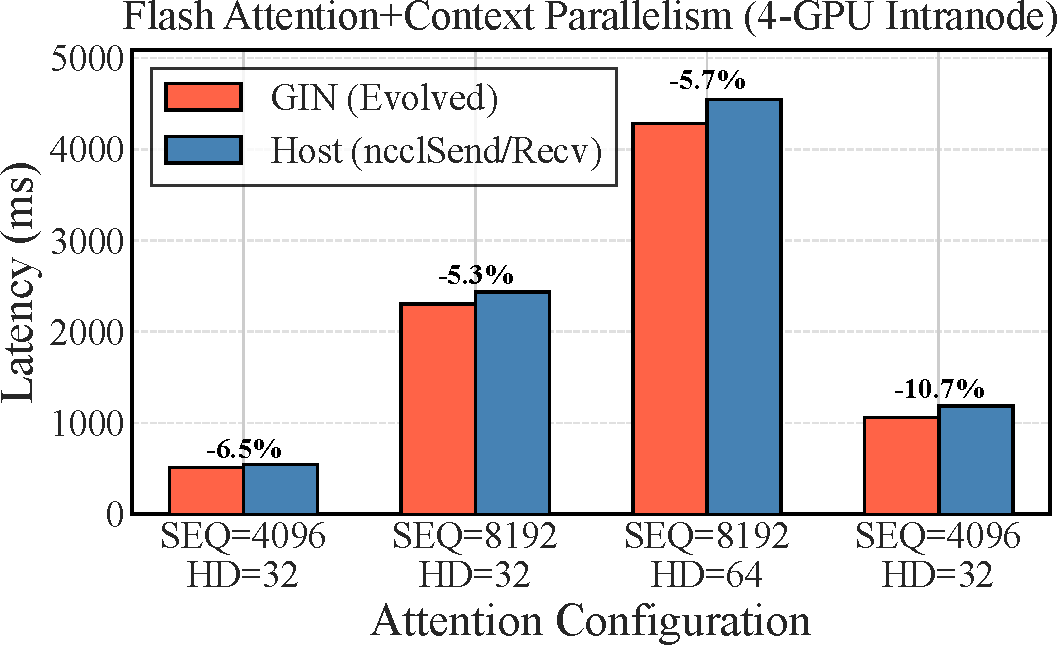
\includegraphics[width=\linewidth]{images/gin_vs_host_bar.pdf}
    \captionof{figure}{\small{Flash Attention with Context Parallelism with varying sequence length and attention head dimension.}}
    \label{fig:flash-attn}
\end{minipage}
\hfill
\begin{minipage}[t]{0.24\textwidth}
    \centering
    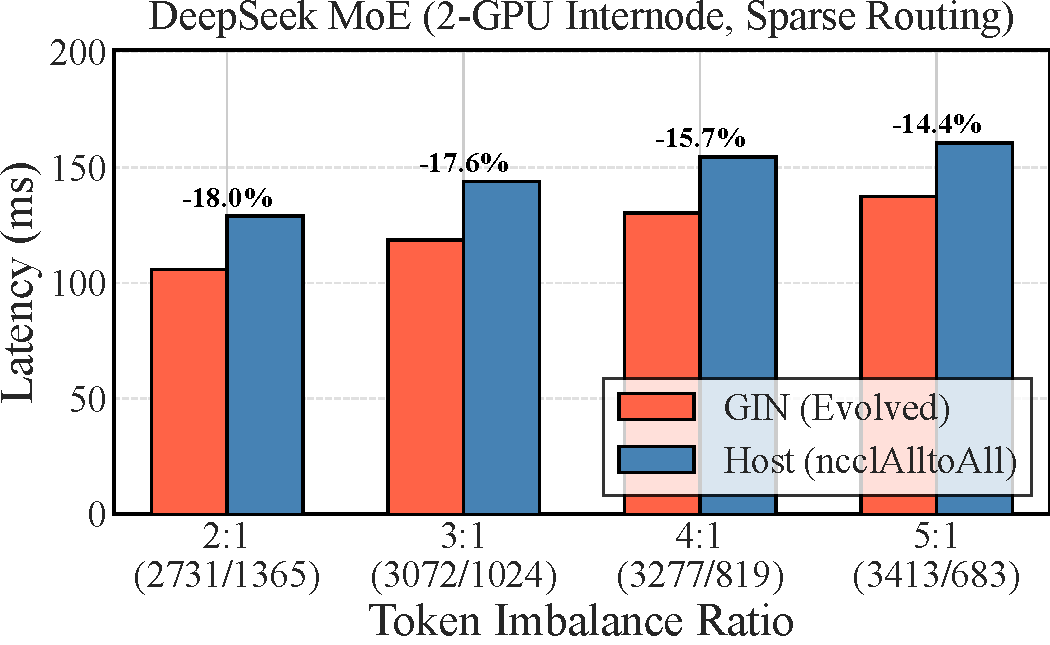
\includegraphics[width=\linewidth]{images/moe_ratio_sweep.pdf}
    \captionof{figure}{\small{DeepSeek-V3 MoE layer across inter-node RoCE links with expert skewness.}}
    \label{fig:moe}
\end{minipage}
\hfill
\begin{minipage}[t]{0.24\textwidth}
    \centering
    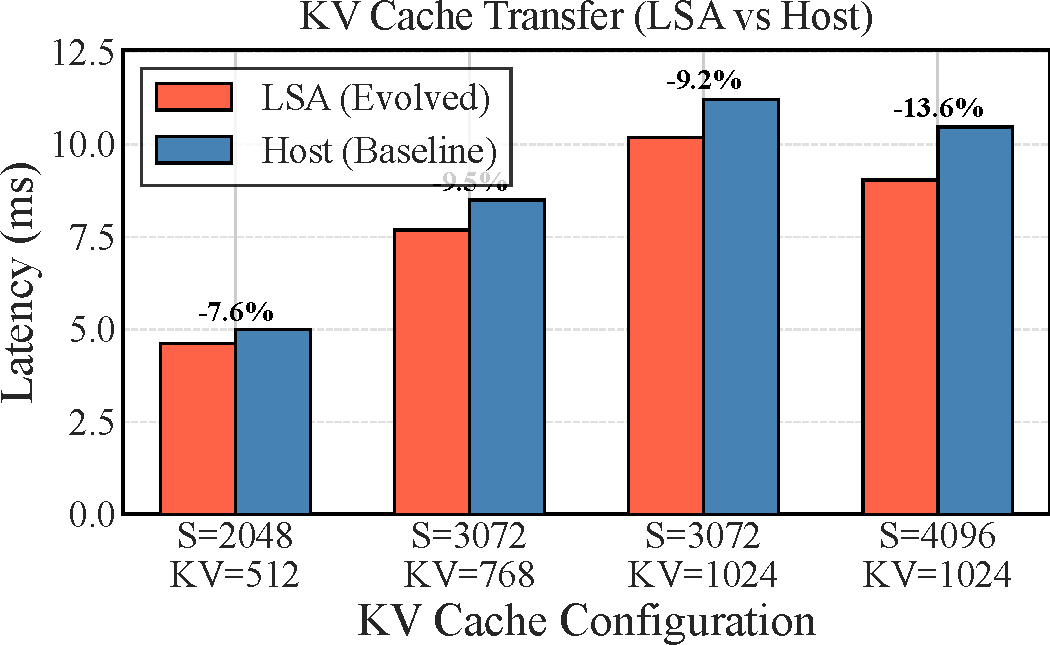
\includegraphics[width=\linewidth]{images/kv_transfer.pdf}
    \captionof{figure}{\small{Intra-node KV cache transfer latency across varying sequence lengths and KV dimensions.}}
    \label{fig:kv-cache}
\end{minipage}
\hfill
\begin{minipage}[t]{0.24\textwidth}
    \centering
    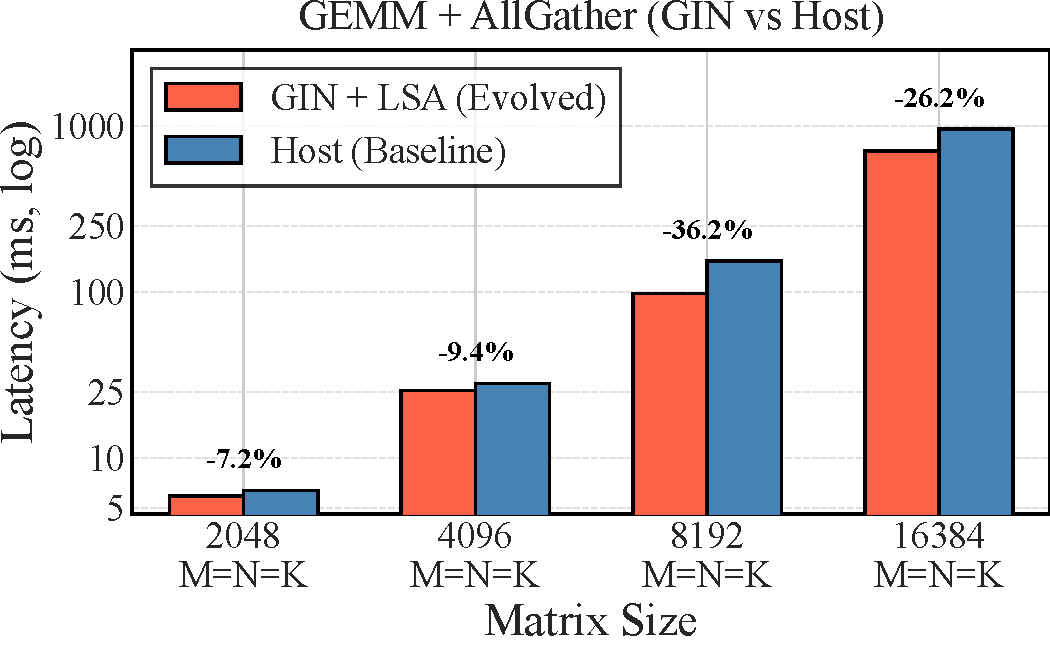
\includegraphics[width=\linewidth]{images/gemm_allgather.pdf}
    \captionof{figure}{\small{Intra- and inter-node GEMM + AllGather latency across square matrix sizes.}}
    \label{fig:gemm-allgather}
\end{minipage}
% \vspace{-8pt}
\end{figure*}

\begin{figure*}[t]
\centering
\setlength{\abovecaptionskip}{0pt}
\setlength{\belowcaptionskip}{-10pt}
\begin{minipage}[t]{0.44\textwidth}
    \centering
    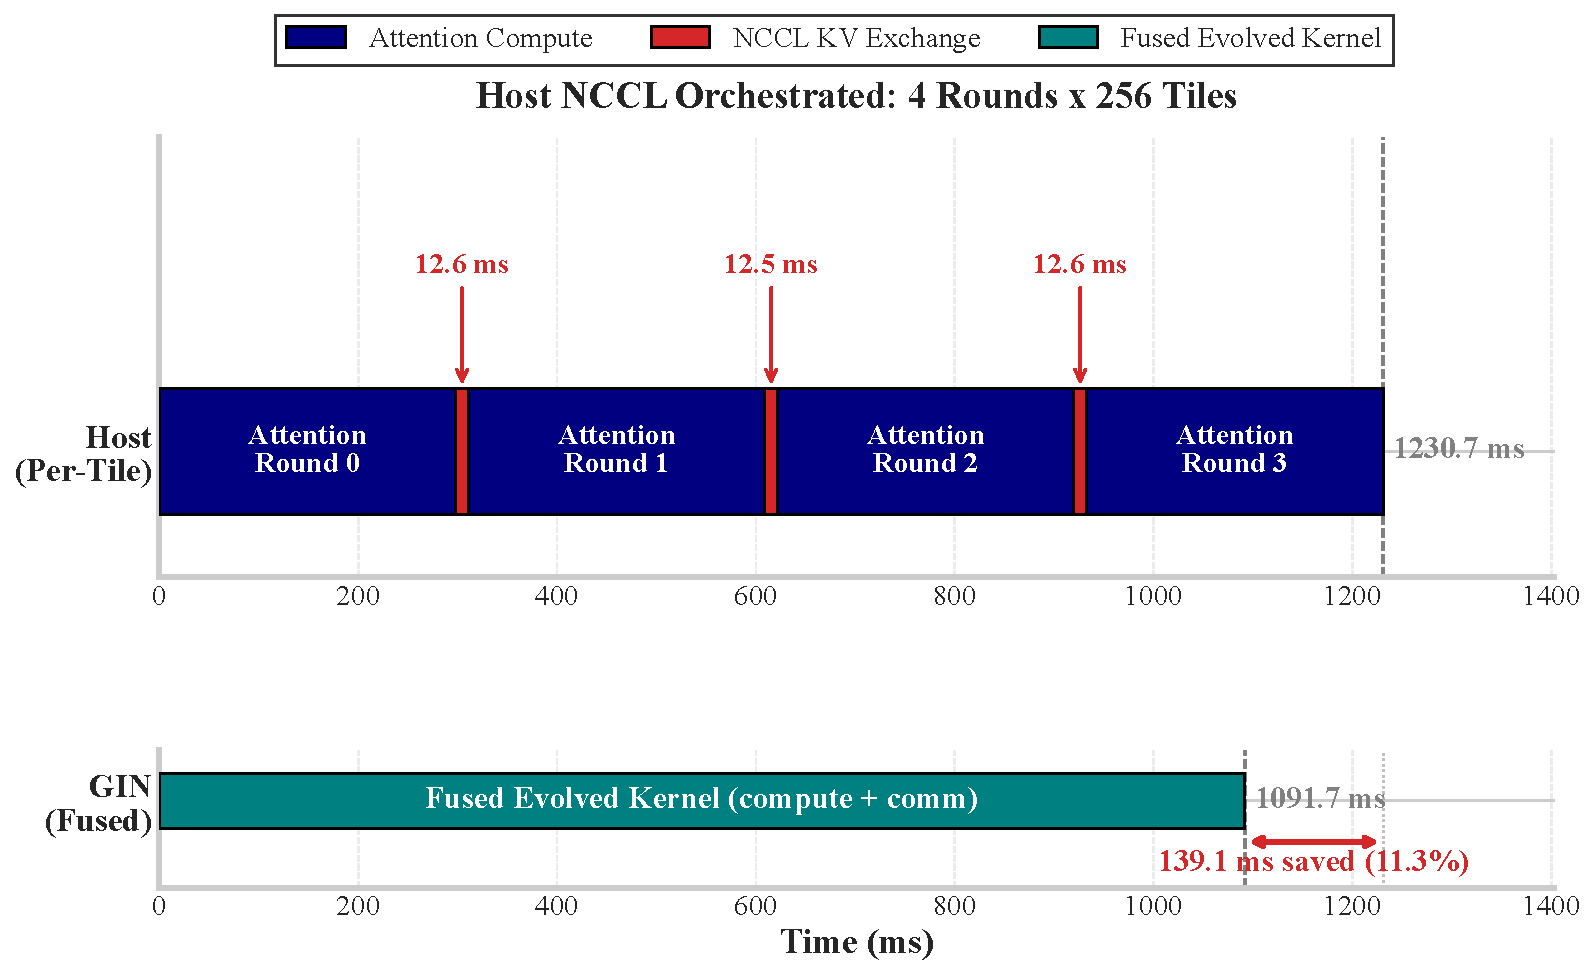
\includegraphics[width=\linewidth]{images/flash_attn_timeline.pdf}
    \captionof{figure}{\small{Flash Attention timeline: host NCCL baseline vs.\ \cufuse{} fused kernel ($\text{SEQ}=4096$, $\text{HD}=32$, 4~GPUs, NVLink). }}
    \label{fig:flash-attn-timeline}
\end{minipage}\hfill
\begin{minipage}[t]{0.55\textwidth}
    \centering
    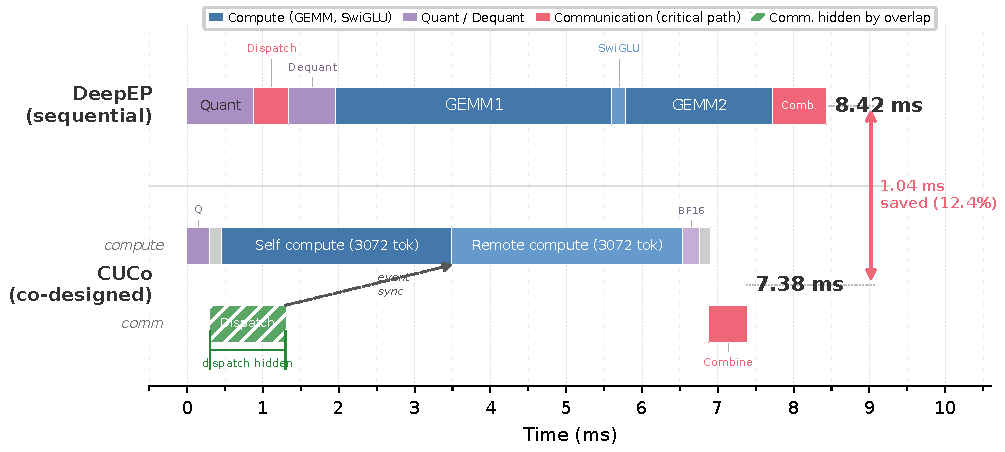
\includegraphics[width=\linewidth]{images/deepep_timeline.pdf}
\captionof{figure}{\small{\textbf{DeepEP vs.\ \cufuse{}} on the MoE layer (Rank~0, 6144 tokens). DeepEP runs phases sequentially. \cufuse{} hides dispatch behind self-compute via a two-stream split.}}
    \label{fig:deepep-timeline}
\end{minipage}
\vspace{-6pt}
\end{figure*}

\vspace{-3pt}
\subsection{\cufuse{}'s End-to-End Evaluation}
\vspace{-3pt}
\label{sec:e2e}

Figures~\ref{fig:flash-attn}--\ref{fig:gemm-allgather} report end-to-end latency for all four workloads. We compare \cufuse{}-evolved device-initiated CUDA against the host-driven NCCL baseline described above; latency is the median over five stable runs measured with CUDA events. Across the reported configurations, \cufuse{} lowers latency by 5.3\%--36.2\% relative to that baseline; our best reported configuration reaches up to $1.57\times$ speedup over host-driven NCCL, consistent with Section~1 and the abstract. The gains stem from fine-grained overlap (e.g., per-tile pipelining, dispatch hiding) that masks network latency behind computation, achieving tight interleavings impossible under host-level orchestration.

\vspace{-3pt}
\subsection{Case Study: Flash Attention with Context Parallelism}
\vspace{-3pt}
\label{sec:flash-attn-deep-dive}

The Flash Attention workload provides a clear demonstration of \cufuse{}'s architectural advantage because the ring structure amplifies per-round overheads across multiple exchange steps. We focus on the configuration ($\text{SEQ}=4096$, $\text{HD}=32$), which exhibits the largest speedup (\textbf{11.3\%}), and use Nsight Systems profiling to dissect where the gains originate. Figure~\ref{fig:flash-attn-timeline} shows the execution timelines.

The \cufuse{} evolved kernel launches a single cooperative grid with a dedicated \emph{communication block} that runs the entire ring protocol (GIN put/wait/flush across all exchange rounds) and separate \emph{compute blocks} that process attention tiles. The critical capability is \emph{per-tile pipelining}: as the comm block completes the transfer of tile~$j$, compute blocks immediately begin processing it---even while later tiles are still in flight. Host orchestration cannot achieve this: because the attention kernel saturates all SMs, a signaling kernel on the communication stream can never be scheduled, creating a priority inversion that forces purely sequential execution between exchange rounds.

As shown in Figure~\ref{fig:flash-attn-timeline}, per-tile pipelining contributes the largest savings (63.7\,ms), followed by eliminating compute-stream idle time during exchange rounds (37.7\,ms) and removing host proxy overhead (37.6\,ms). Together, these reduce end-to-end latency from \textbf{1230.7\,ms} to \textbf{1091.7\,ms}. Full architectural details (block counts, double-buffering, synchronization primitives) are in Appendix~\ref{sec:flash_attn_details}.


\vspace{-3pt}
\subsection{Comparison with Expert-Crafted Libraries}
\vspace{-3pt}
\label{sec:deepep-comparison}

\noindent\textbf{Why DeepEP (and not every expert stack).}
Among recent industrial stacks~\cite{deepep2025, chang2024flux, licker2025rdmap2p}, DeepEP was the only library we could install, run, and profile end-to-end on our hardware (A100, NVLink intra-node, RoCE inter-node). It ships optimized transports and exposes async APIs (\texttt{async\_finish}, \texttt{previous\_event}, dedicated comm stream) that could enable overlap---but as a \emph{communication primitive library}, it leaves higher-level co-design decisions to the caller, precisely the layer \cufuse{} automates. We evaluate on the DeepSeek-V3 MoE layer (2 A100 GPUs, intranode NVLink, 4096 tokens, TF32 compute) using DeepEP's standard sequential single-stream flow. Table~\ref{tab:deepep-comparison} shows the per-phase breakdown.

\begin{figure*}[t]
\begin{minipage}[c]{0.58\textwidth}
\centering
\scriptsize
\setlength{\tabcolsep}{4pt}
\captionof{table}{Per-phase latency: DeepEP vs.\ \cufuse{} on the DeepSeek-V3 MoE layer (2~A100s, NVLink, Rank~0, 6144 tokens).}
\vspace{4pt}
\label{tab:deepep-comparison}
\begin{tabular}{lrrr}
\toprule
\textbf{Phase} & \textbf{DeepEP (ms)} & \textbf{\cufuse{} (ms)} & $\boldsymbol{\Delta}$ \textbf{(ms)} \\
\midrule
FP8 quantize              & 0.88 & 0.30 & $-$0.58 \\
Dispatch (comm)            & 0.47 & ${\sim}$1.0\textsuperscript{$\dagger$} & \emph{hidden} \\
Compute\textsuperscript{$\ddagger$} & 6.38 & 6.08 & $-$0.30 \\
BF16 cast + overhead       & ---  & 0.30 & +0.30 \\
Combine (comm)             & 0.68 & ${\sim}$0.70 & +0.02 \\
\midrule
\textbf{Total (wall clock)} & \textbf{8.42} & \textbf{7.38} & \textbf{$-$1.04} \\
\textbf{Dispatch on crit.\ path} & \textbf{yes} & \textbf{no} & \textbf{$-$12.4\%} \\
\bottomrule
\end{tabular}
\\[2pt]
{\scriptsize $\dagger$~Concurrent with self-compute; hidden behind 3.04\,ms of local-chunk work.}\\
{\scriptsize $\ddagger$~DeepEP: one GEMM (6144 tok). \cufuse{}: two GEMMs (3072+3072), same cuBLAS TF32.}
\end{minipage}\hfill
\begin{minipage}[c]{0.38\textwidth}
\centering
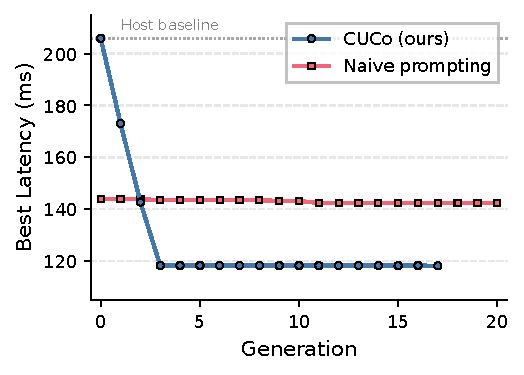
\includegraphics[width=0.92\linewidth]{images/ablation_naive_prompting.pdf}
\vspace{-4pt}
\captionof{figure}{\small{CUCo vs.\ naive iterative prompting on the GIN MoE workload. CUCo reaches 118\,ms by gen.~3; naive prompting plateaus at 142\,ms.}}
\label{fig:ablation-naive}
\end{minipage}
\vspace{-10pt}
\end{figure*}

\noindent\textbf{What \cufuse{} discovered.}
Figure~\ref{fig:deepep-timeline} visualizes the two execution models. The agent's evolutionary search converged on a two-stream overlap pipeline with three co-design decisions: (1)~\emph{self/remote compute split}---recognizing that tokens routed to the local expert can be processed immediately without waiting for the network, the agent splits the single GEMM into two smaller GEMMs (3072 tokens each); (2)~\emph{dispatch hiding}---running the dispatch kernel on a high-priority \texttt{comm\_stream} concurrently with self-chunk compute on a normal-priority \texttt{compute\_stream}, gating remote-chunk compute on dispatch completion via a CUDA event; and (3)~\emph{backend selection}---choosing LSA (direct peer memory stores) over GIN (RDMA-style put/signal) for the NVLink topology. Each decision is a point in the design space $\mathcal{C}$ (Table~\ref{tab:fusion_space}).

\noindent\textbf{Why \cufuse{} wins despite slower raw communication.}
DeepEP's primitives are faster in isolation (0.47\,ms vs.\ ${\sim}$1.0\,ms), but this is irrelevant when dispatch is hidden behind self-compute (3.04\,ms $>$ 1.0\,ms). The 1.04\,ms end-to-end saving corresponds to the dispatch plus quantization overhead that DeepEP exposes sequentially.

\noindent\textbf{Multi-layer scaling.}
Over $L{=}1$ to $16$ consecutive MoE layers, \cufuse{} maintains a stable 12--14\% per-layer advantage (7.29--7.38\,ms vs.\ 8.45--8.50\,ms), confirming that the overlap benefit is structural and per-layer, not a warmup artifact.

% \noindent\textbf{Scope and limitations.}
% DeepEP is \emph{not} inherently sequential---it provides async primitives that an expert could use to construct a similar overlap pipeline. \cufuse{}'s contribution is discovering and implementing this co-design pattern automatically, including the non-obvious self/remote decomposition and backend selection. In communication-dominated regimes where dispatch exceeds compute (e.g., inter-node with small models), DeepEP's faster raw transport would reduce the overlap window---an important direction for future work.

% ============================================================
\vspace{-10pt}
\subsection{Ablation Studies}
\vspace{-10pt}
\label{sec:ablation}
% ============================================================
\noindent\textbf{Fast-Path Agent.}
We evaluate whether the fast-path agent is necessary by comparing the full \cufuse{} pipeline (fast-path + slow-path) against a \emph{slow-path--only} ablation that runs the evolutionary agent directly on the original host NCCL code, bypassing the fast-path transformation entirely. Both configurations use the DeepSeek-V3 MoE workload (2-GPU inter-node, RoCE) with identical LLM models, evaluation harness, and evolutionary budgets.

\begin{figure*}[t]
\centering
\setlength{\abovecaptionskip}{2pt}
\setlength{\belowcaptionskip}{-8pt}
\begin{minipage}[t]{0.24\textwidth}
    \centering
    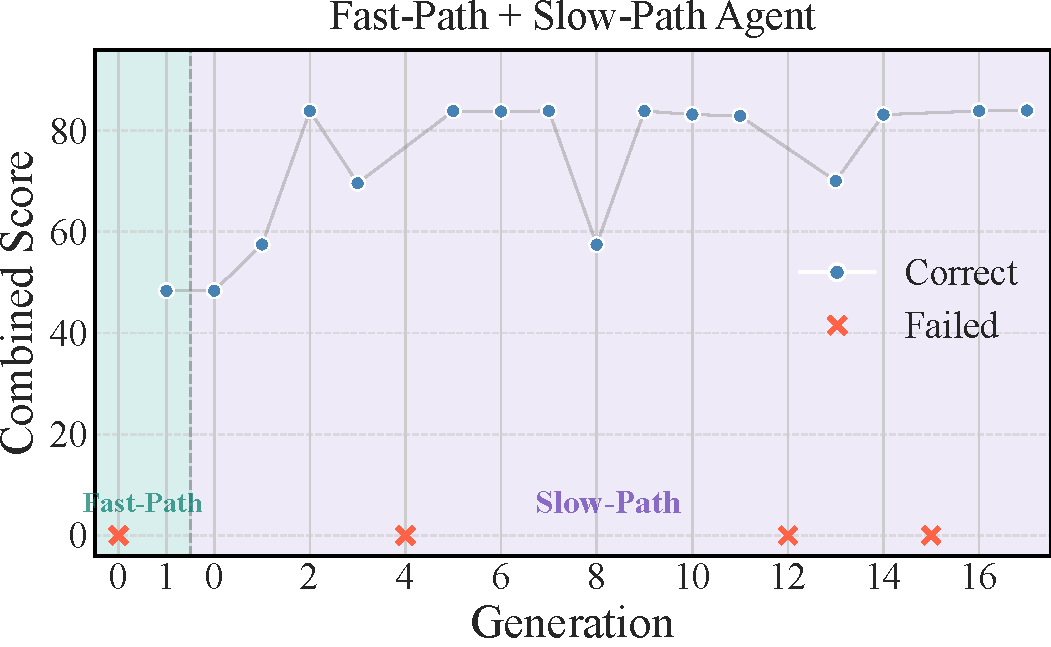
\includegraphics[width=\linewidth]{images/ablation_fast_slow.pdf}
    \captionof{figure}{\small{Fast-path + slow-path agent on the GIN MoE workload.}}
    \label{fig:ablation-fast-slow}
\end{minipage}
\hfill
\begin{minipage}[t]{0.24\textwidth}
    \centering
    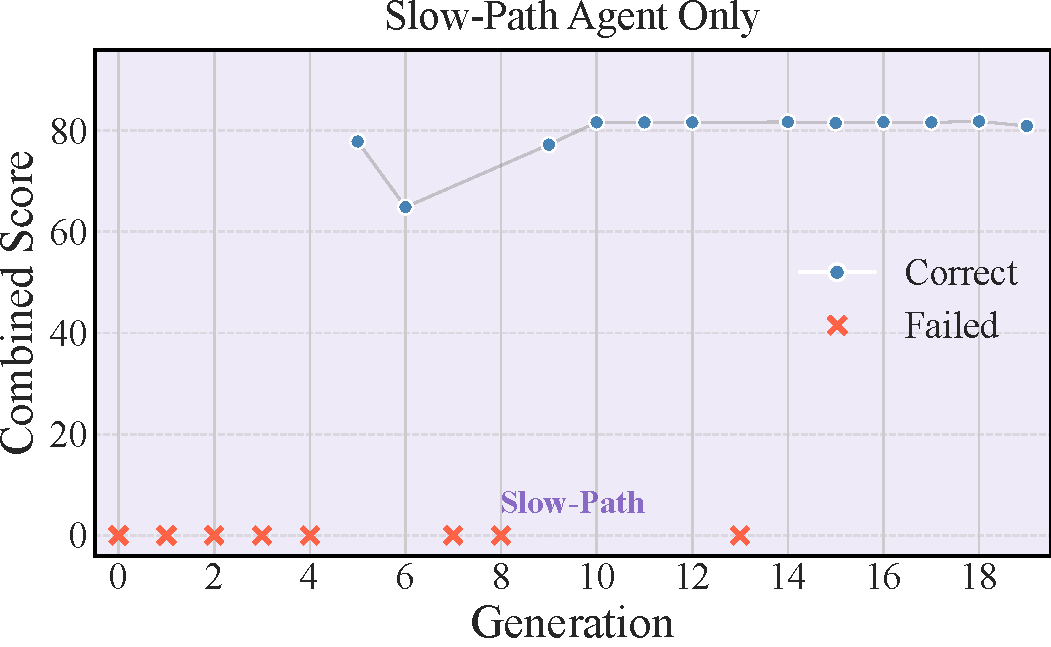
\includegraphics[width=\linewidth]{images/ablation_slow_only.pdf}
    \captionof{figure}{\small{Slow-path agent only on the same workload.}}
    \label{fig:ablation-slow-only}
\end{minipage}
\hfill
\begin{minipage}[t]{0.24\textwidth}
    \centering
    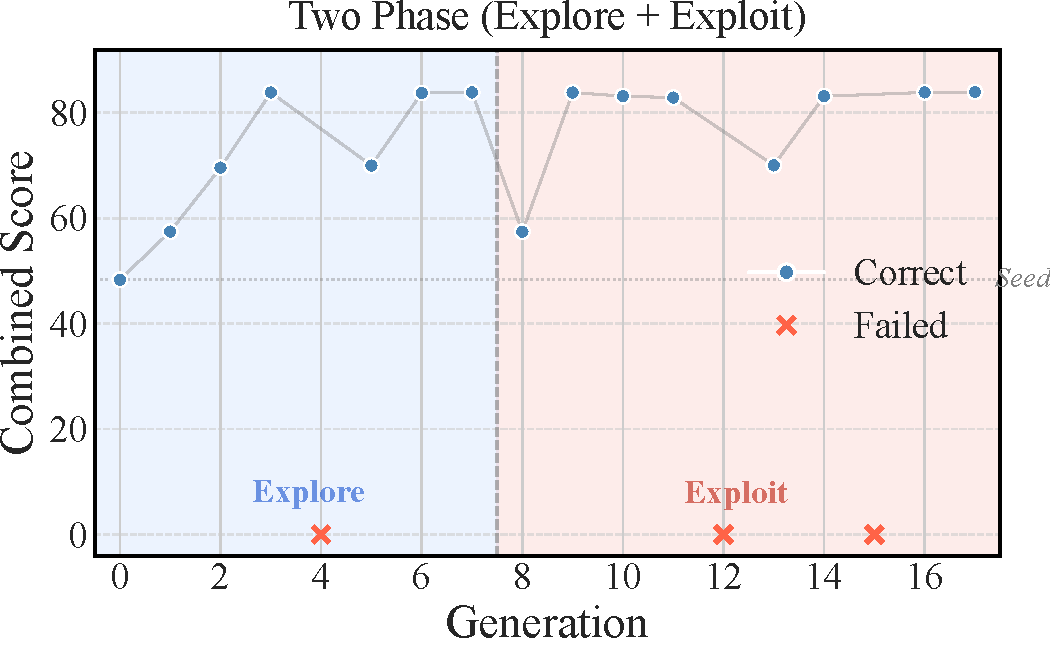
\includegraphics[width=\linewidth]{images/evolution_plot_2_phase.pdf}
    \captionof{figure}{\small{Two-phase evolution (explore-exploit) on the MoE workload.}}
    \label{fig:evo-two-phase}
\end{minipage}
\hfill
\begin{minipage}[t]{0.24\textwidth}
    \centering
    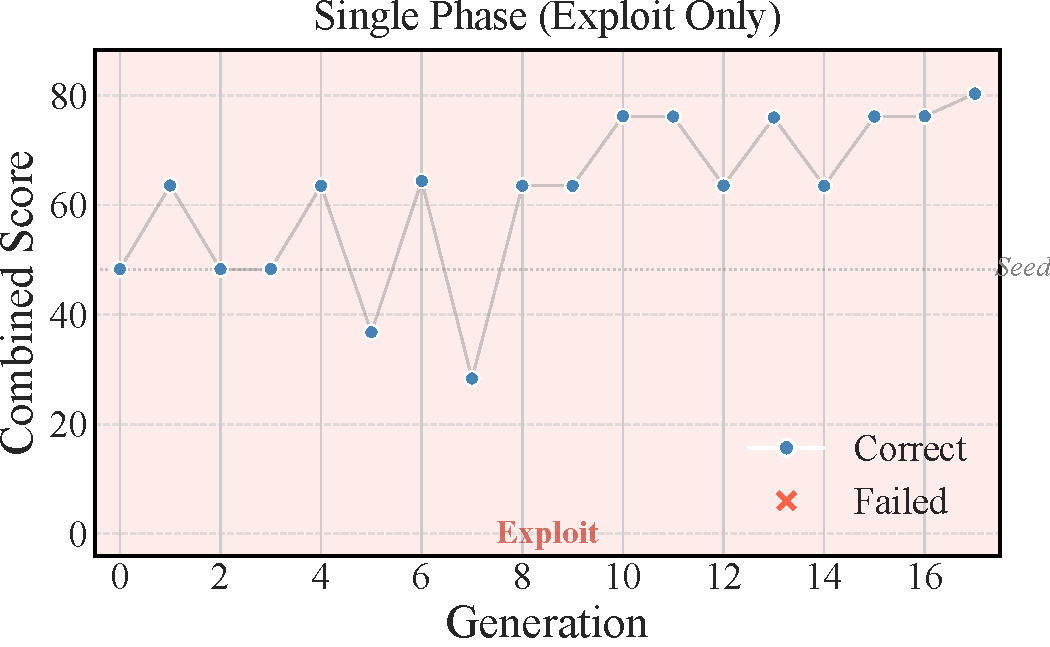
\includegraphics[width=\linewidth]{images/evolution_plot_1_phase.pdf}
    \captionof{figure}{\small{Single-phase evolution (exploit only) on the same workload.}}
    \label{fig:evo-single-phase}
\end{minipage}
\vspace{-12pt}
\end{figure*}

Figures~\ref{fig:ablation-fast-slow} and~\ref{fig:ablation-slow-only} show the results. With the fast-path agent, a correct GIN kernel emerges in 2~LLM iterations (score 48.34), and the slow-path reaches \textbf{83.95} within 3~generations. Without it (Figure~\ref{fig:ablation-slow-only}), the evolutionary agent must discover the GIN programming model while simultaneously optimizing---the first 5~generations all fail (compilation errors, deadlocks), wasting 25\% of the budget. It does not stabilize above 81 until generation~10 and peaks at \textbf{81.81}---\textbf{2.5\% lower}. The fast-path decomposition avoids wasting early generations on infrastructure discovery.

\noindent\textbf{Explore-Exploit Phases.}
We compare a \emph{two-phase} schedule (40\% explore then exploit) against \emph{single-phase} exploit-only, both on the GIN MoE workload with 18~generations. The two-phase schedule (Figure~\ref{fig:evo-two-phase}) reaches 83.86 by generation~3 and peaks at \textbf{83.95}. The exploit-only schedule (Figure~\ref{fig:evo-single-phase}) oscillates for 9~generations, exceeds 76 only at generation~10, and peaks at 80.36---a \textbf{4.3\% lower final score}. The explore phase discovers structurally diverse strategies (barrier-free overlap, split put/wait, signal-shadow synchronization) that the exploit phase refines; without this diversity, the agent converges slowly to a local optimum.

\noindent\textbf{Naive Iterative Prompting.}
We compare against iterative prompting without population, crossover, or meta-recommendations on the same GIN MoE workload (Figure~\ref{fig:ablation-naive}). Over 20~generations, naive prompting improves by only 1.1\% (144$\to$142.3\,ms), plateauing after generation~11. \cufuse{} reaches 118.1\,ms within 3~generations---a \textbf{17\% improvement}---confirming the value of population-based search over single-program refinement.

\vspace{-8pt}
\section{Conclusion}
\vspace{-8pt}
\cufuse{} automates compute-communication co-design by constraining an LLM agent to a structured configuration space rather than unconstrained code generation, separating correctness (fast-path transformation to a verified seed) from performance (evolutionary search), and injecting hardware context so the same pipeline adapts across topologies. Across four multi-GPU workloads, \cufuse{} delivers up to $1.57\times$ speedup over host-driven baselines and a 12--14\% per-layer advantage over standard DeepEP usage on intranode MoE. These results suggest that LLM agents are most effective as bounded variation operators over domain-defined spaces, and that correctness-first decomposition is essential to avoid wasting search budget on broken candidates.

% \noindent\textbf{Ethics}: This work does not raise any ethical issues.

% \section*{Acknowledgments}
% We gratefully acknowledge the generous support of Google, Meta, and Cisco, whose funding made this research possible. We thank the members of the UT Networked Systems research group for insightful discussions and constructive feedback throughout the development of this work.
